% Figure from MATH 556 notes, section 22. Compile with the notes preamble.
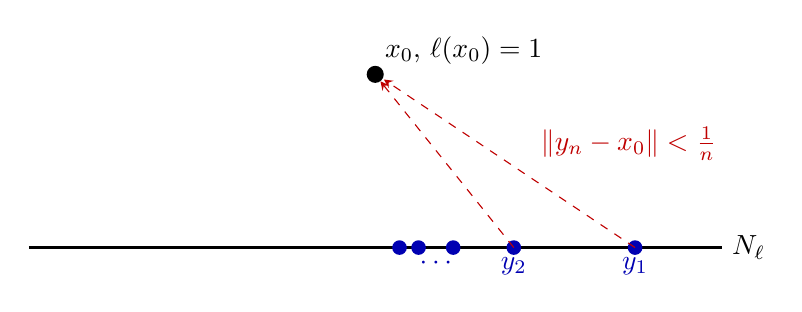
\begin{tikzpicture}[scale=2.2, >=stealth]
    \draw[thick] (-0.8,0) -- (3.2,0) node[right] {$N_\ell$};
    \fill (1.2,1) circle (1.4pt) node[above right] {$x_0$, $\ell(x_0) = 1$};
    \foreach \n/\x in {1/2.7,2/2.0,3/1.65,4/1.45,5/1.34} {\fill[blue!70!black] (\x,0) circle (1.2pt);}
    \node[blue!70!black, below] at (2.7,0) {$y_1$}; \node[blue!70!black, below] at (2.0,0) {$y_2$}; \node[blue!70!black, below] at (1.55,0) {$\cdots$};
    \draw[->, dashed, red!75!black] (2.7,0) -- (1.25,0.97);
    \draw[->, dashed, red!75!black] (2.0,0) -- (1.23,0.96);
    \node[red!75!black, right] at (2.1,0.6) {$\|y_n - x_0\| < \frac1n$};
\end{tikzpicture}
